\documentclass[11pt,a4paper]{article}
\usepackage[utf8]{inputenc}
\usepackage[T1]{fontenc}
\usepackage[portuguese]{babel}
\usepackage[a4paper, margin=1.8cm, top=1.5cm, bottom=1.5cm]{geometry}
\usepackage{graphicx}
\usepackage[hidelinks]{hyperref}
\usepackage{enumitem}
\usepackage{titlesec}
\usepackage{xcolor}
\usepackage{amsmath,amssymb}

% Formatação de seções
\titleformat{\section}{\large\bfseries\color{darkgray}}{}{0em}{}[\titlerule]
\titlespacing{\section}{0pt}{1.3ex}{0.8ex}

\begin{document}
\pagestyle{empty}

\begin{minipage}[c]{0.75\textwidth}
    {\Huge \bfseries Matheus Sousa} \\[0.35cm]
    Paudalho, PE, Brasil \\
    Telefone: (81) 98910-6565 \\
    Email: \href{mailto:matheuzinhorxoficial@gmail.com}{matheuzinhorxoficial@gmail.com} \\
    LinkedIn: \href{https://www.linkedin.com/in/matheus-sousa-739893255/}{https://www.linkedin.com/in/matheus-sousa-739893255/} \\
    GitHub: \href{https://github.com/Matheuzinh0}{https://github.com/Matheuzinh0}
\end{minipage}
\begin{minipage}[c]{0.2\textwidth}
    \begin{flushright}
        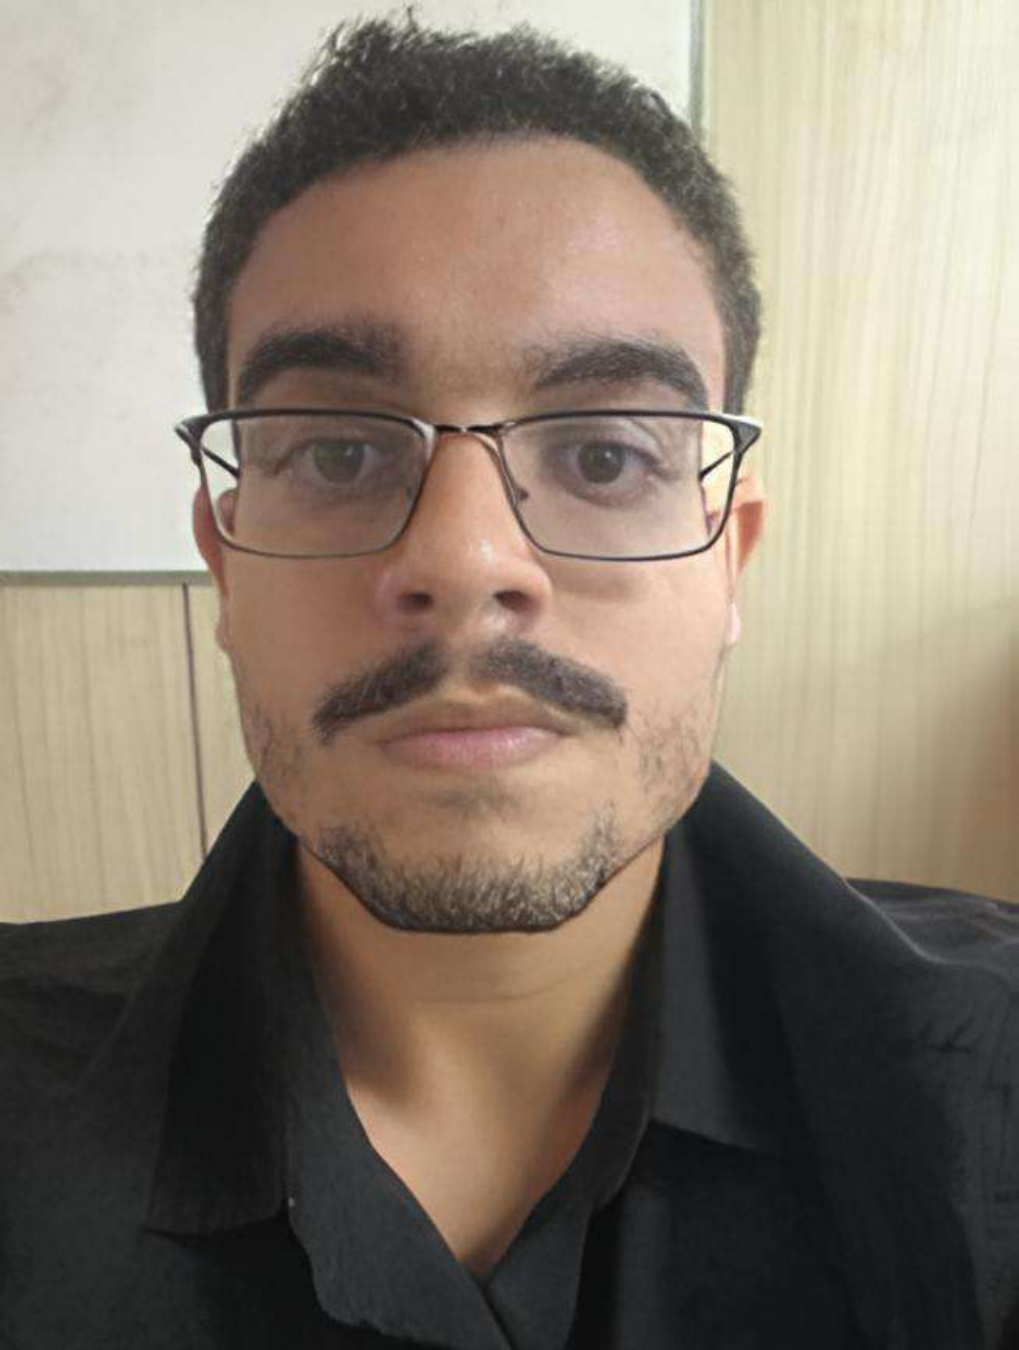
\includegraphics[width=3cm, height=3.8cm, keepaspectratio]{foto.jpg}
    \end{flushright}
\end{minipage}

\vspace{0.3cm}

\section*{Resumo Profissional}
Estudante de Engenharia de Telecomunicações na UFPE (8º período) e Técnico em ADS, com atuação voltada a Cibersegurança, Criptoanálise e Segurança de Hardware/Firmware. Pesquisador em criptoanálise formal (linear e diferencial) de cifras de fluxo e concepção de primitivas criptográficas em hardware (FPGA) e software (C/C++, Python). Experiência na identificação de vulnerabilidades algorítmicas, validação adversarial com baterias estatísticas (NIST SP 800-22), desenvolvimento de firmware de tempo real para microcontroladores (ESP32, STM32) e análise de tráfego de redes (Wireshark). Perfil altamente analítico com sólida fundamentação matemática (medalhista OBM), direcionado à segurança ofensiva e defensiva de sistemas críticos.

\section*{Formação Acadêmica}
\textbf{Universidade Federal de Pernambuco (UFPE)} \hfill Recife, PE \\
Bacharelado em Engenharia de Telecomunicações \hfill \textit{Previsão de conclusão: 2028} \\
\textit{Atual: 8º Período}

\vspace{0.2cm}

\textbf{Escola Técnica Estadual Senador Wilson Campos (ETE-SWC)} \hfill Paudalho, PE \\
Técnico em Análise e Desenvolvimento de Sistemas \hfill \textit{2019}

\section*{Iniciação Científica e Pesquisa em Segurança}

\textbf{Iniciação Científica (PIBIC/CNPq) -- Criptoanálise de Cifras de Fluxo} \hfill UFPE \\
\textit{Laboratório de Comunicação e Segurança da Informação (LCSI)} \hfill \textit{2026 -- Presente} \\
\textit{Plano: Estratégias de Criptoanálise Aplicadas a Cifras de Fluxo sobre Anéis de Inteiros} \\
\textit{Orientador: Prof. Dr. Daniel Pedro Bezerra Chaves}
\begin{itemize}[leftmargin=*, noitemsep]
    \item Modelagem e implementação de ataques de criptoanálise diferencial e linear contra cifras de fluxo e geradores pseudoaleatórios (PRNGs) sobre anéis de inteiros ($\mathbb{Z}_{2^m}$) frente a modelos adversariais formais.
    \item Avaliação de segurança adversarial via propagação de diferenças controladas em chaves, vetores de inicialização (IV) e estado interno, quantificando taxas de avalanche, pesos de Hamming e distinguidores estatísticos.
    \item Investigação de correlações e aproximações lineares fundamentadas em espectro de Walsh para identificação de vieses estruturais exploráveis por atacantes computacionalmente limitados.
    \item Concepção e validação computacional de contramedidas por meio de funções de pós-processamento não linear de baixa complexidade (operações modulares, rotações e XORs), preservando a viabilidade de síntese em FPGA.
\end{itemize}

\vspace{0.25cm}

\textbf{Iniciação Científica -- Criptografia em Hardware e Primitivas Seguras} \hfill UFPE \\
\textit{Laboratório de Comunicação e Segurança da Informação (LCSI)} \hfill \textit{2025 -- 2026} \\
\textit{Orientador: Prof. Dr. Daniel Pedro Bezerra Chaves}
\begin{itemize}[leftmargin=*, noitemsep]
    \item Pesquisa e implementação de geradores de números pseudoaleatórios (PRNG) de alto throughput e cifras simétricas em C/C++, aplicando mapas caóticos discretos (\textit{Arnold's Cat Map}) e corpos finitos $\mathrm{GF}(2^e)$.
    \item Síntese de circuitos e prototipagem em FPGA (AMD/Xilinx) utilizando linguagens Verilog e VHDL, focando em segurança arquitetural, otimização de área lógica e imunidade a gargalos de temporização.
    \item Validação de propriedades estatísticas e conformidade criptográfica através de baterias padronizadas (NIST SP 800-22 e TestU01), com resultados publicados em periódico internacional indexado.
\end{itemize}

\newpage

\section*{Projetos de Engenharia e Sistemas de Segurança}

\textbf{Comunicação Crítica e Firmware Seguro para Robótica (SSL)} \hfill \textit{Projeto Acadêmico}
\begin{itemize}[leftmargin=*, noitemsep]
    \item Desenvolvimento de firmware em C/C++ sobre microcontroladores ESP12F/ESP32 para comunicação sem fio de ultrabaixa latência em robôs móveis autônomos da categoria SSL.
    \item Estruturação de protocolos de transmissão, empacotamento seguro e rotinas de validação de comandos em tempo real entre a estação base e agentes móveis integrados a sistemas de visão computacional.
    \item Análise de integridade de sinais em nível de barramento de hardware com osciloscópio e multímetro, combinada a análise de vulnerabilidades de rede e tráfego RF.
\end{itemize}

\vspace{0.25cm}

\textbf{Infraestrutura Segura de Alto Desempenho e Criptografia Leve} \hfill \textit{Projetos Independentes}
\begin{itemize}[leftmargin=*, noitemsep]
    \item Desenvolvimento de cluster computacional com CPUs Intel Xeon gerenciado via \textit{Slurm} para paralelismo e orquestração de testes massivos de simulação e criptoanálise.
    \item Estudo e implementação de cifras de fluxo para ambientes restritos (SNOW 3G) e modos autenticados (AES-128-GCM em C), avaliando trade-offs entre segurança e consumo de recursos.
\end{itemize}

\section*{Habilidades Técnicas}
\begin{itemize}[leftmargin=*, noitemsep]
    \item \textbf{Cibersegurança e Criptografia:} Criptoanálise linear e diferencial, análise de vulnerabilidades, cifras de fluxo e bloco (AES-128-GCM), CSPRNGs, análise espectral (Walsh), testes estatísticos (NIST SP 800-22, TestU01).
    \item \textbf{Segurança de Hardware e Embarcados:} FPGA (AMD Vivado, Intel Quartus Prime, Verilog, VHDL), microcontroladores (ESP32/ESP12F, STM32), análise de barramentos físicos (UART, SPI, I2C, RF), firmware seguro.
    \item \textbf{Linguagens de Programação:} C/C++ avançado (manipulação de bits, ponteiros, baixo nível, performance), Python (automação, scripts de validação e exploração).
    \item \textbf{Redes, Sistemas e Ferramentas:} Análise de tráfego de rede (Wireshark, TCP/IP), Linux avançado (Ubuntu, Manjaro), Shell Scripting (Bash), orquestração Slurm, Git para versionamento, instrumentação (osciloscópio, multímetro).
\end{itemize}

\section*{Publicações Científicas}
\begin{itemize}[leftmargin=*, noitemsep]
    \item SOUZA, C. E. C.; MORENO, D.; \textbf{SOUSA, M. H. S.}; CHAVES, D. P. B.; PIMENTEL, C. High-Throughput Pseudo-Random Number Generators Over Discrete Chaos. \textit{IEEE Transactions on Circuits and Systems II: Express Briefs}, v. 72, n. 9, p. 1303--1307, 2025.
    \item DELGADO NETO, A. S.; SOUZA, C. E. C.; ALMEIDA, D. C. M.; \textbf{SOUSA, M. H. S.}; CHAVES, D. P. B.; PIMENTEL, C. Geradores de Números Pseudo-Aleatórios baseados em Recorrências Lineares sobre $\mathrm{GF}(2^e)$. In: \textit{XLIII Simpósio Brasileiro de Telecomunicações e Processamento de Sinais (SBrT)}, 2025.
\end{itemize}

\section*{Certificações e Premiações}
\begin{itemize}[leftmargin=*, noitemsep]
    \item \textbf{Medalhista de Bronze -- 6ª Competição Elon Lages Lima (OBM):} Associação Olimpíada Brasileira de Matemática (2025).
    \item \textbf{Olimpíada Brasileira de Matemática Universitária (OBMU):} Participação na edição de 2025.
    \item \textbf{Certificado de Operador de Estação de Radioamador (COER) - Classe B:} Expedido pela Anatel (2025). Conhecimentos práticos em antenas e transceptores.
\end{itemize}

\end{document}
